\documentclass[border=4pt]{standalone}
\usepackage{tikz}
\usetikzlibrary{positioning, arrows.meta, shapes.geometric, calc, fit, backgrounds}
\usepackage{amsmath,amssymb}
\begin{document}
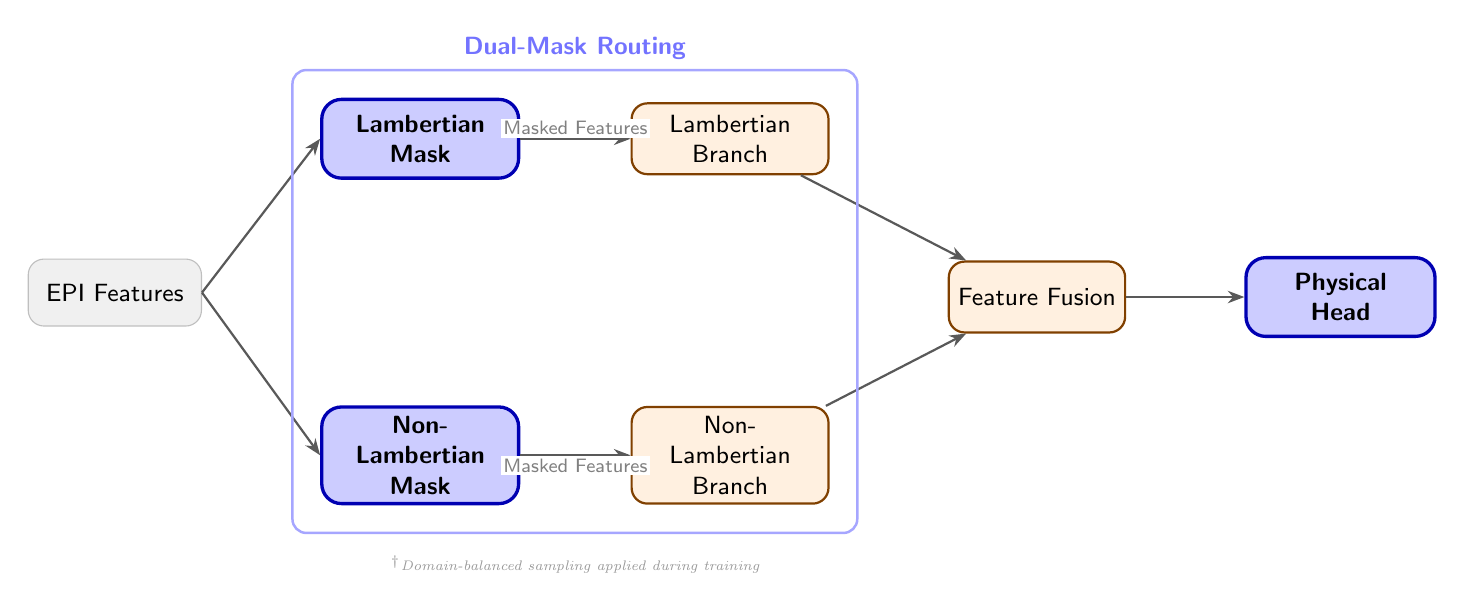
\begin{tikzpicture}[
  input/.style={draw, rounded corners=2mm, minimum width=2.2cm, minimum height=0.85cm,
                fill=gray!12, draw=gray!50, align=center, font=\sffamily\small},
  innov/.style={draw, rounded corners=2.5mm, minimum width=2.5cm, minimum height=1.0cm,
                fill=blue!20, draw=blue!70!black, line width=1.2pt, align=center,
                font=\sffamily\small\bfseries, text width=2.0cm},
  proc/.style={draw, rounded corners=2mm, minimum width=2.5cm, minimum height=0.9cm,
               fill=orange!12, draw=orange!50!black, line width=0.8pt, align=center,
               font=\sffamily\small, text width=2.0cm},
  fusion/.style={draw, rounded corners=2mm, minimum width=2.2cm, minimum height=0.9cm,
                 fill=orange!12, draw=orange!50!black, line width=0.8pt, align=center,
                 font=\sffamily\small},
  output/.style={draw, rounded corners=2.5mm, minimum width=2.4cm, minimum height=1.0cm,
                 fill=blue!20, draw=blue!70!black, line width=1.2pt, align=center,
                 font=\sffamily\small\bfseries, text width=2.0cm},
  arr/.style={-{Stealth[length=6pt]}, thick, color=black!65},
  lbl/.style={font=\sffamily\scriptsize, text=black!50, fill=white, inner sep=1pt},
  gbox/.style={draw=blue!35, rounded corners=5pt, inner sep=10pt, line width=0.9pt},
]

% Input
\node[input] (m1) {EPI Features};

% Dual Masks (innovation modules)
\node[innov, above right=1.0cm and 1.5cm of m1] (m2) {Lambertian Mask};
\node[innov, below right=1.0cm and 1.5cm of m1] (m3) {Non-Lambertian Mask};

% Processing Branches
\node[proc, right=1.4cm of m2] (m4) {Lambertian Branch};
\node[proc, right=1.4cm of m3] (m5) {Non-Lambertian Branch};

% Feature Fusion - centered between branches
\path (m4.east) -- (m5.east) coordinate[midway] (midbr);
\node[fusion, right=1.5cm of midbr, anchor=west] (m6) {Feature Fusion};

% Physical Head (innovation output)
\node[output, right=1.5cm of m6] (m7) {Physical Head};

% Main flow arrows
\draw[arr] (m1.east) -- (m2.west);
\draw[arr] (m1.east) -- (m3.west);
\draw[arr] (m2) -- node[lbl, above] {Masked Features} (m4);
\draw[arr] (m3) -- node[lbl, below] {Masked Features} (m5);
\draw[arr] (m4) -- (m6);
\draw[arr] (m5) -- (m6);
\draw[arr] (m6) -- (m7);

% Grouping box - Dual-Mask Routing
\node[gbox, fit=(m2)(m3)(m4)(m5),
      label={[font=\sffamily\small\bfseries, text=blue!55]above:Dual-Mask Routing}] (gbox1) {};

% Training annotation
\node[font=\tiny\itshape, text=black!40, below=0.15cm of gbox1.south, anchor=north]
      {$^\dagger$Domain-balanced sampling applied during training};

\end{tikzpicture}
\end{document}